\documentclass[landscape,a0paper,25pt,margin=0mm]{tikzposter}

%%%%%%%%%%%%%%%%%%%%%%%%%%%%%%%%%%%%%%%%%%%%%%%%%%%%%%%%%%%%%%%%%%%%%%%%%
%    UU STYLING
%%%%%%%%%%%%%%%%%%%%%%%%%%%%%%%%%%%%%%%%%%%%%%%%%%%%%%%%%%%%%%%%%%%%%%%%%
\tikzposterlatexaffectionproofoff

% UU wants arial font. Helvetica is close enough
\usepackage{helvet} 
\renewcommand{\familydefault}{\sfdefault}

% https://tex.stackexchange.com/questions/180234/how-can-i-make-my-title-wrap-in-a-tikzposter
% \makeatletter
% \def\title#1{\gdef\@title{\scalebox{\TP@titletextscale}{%
% \begin{minipage}[t]{\linewidth}
% \centering
% #1
% \par
% \vspace{0.5em}
% \end{minipage}%
% }}}
% \makeatother


% Profile colors according to 
% https://mp.uu.se/en/web/info/stod/kommunikation-riktlinjer/grafiskariktl/profilfarger
\definecolor{uured}{RGB}{153,0,0}
\definecolor{uudarkgrey}{RGB}{130,130,130}
\definecolor{uumidgrey}{RGB}{190,190,190}
\definecolor{uulightgrey}{RGB}{230,230,230}
\definecolor{uuPosterBorder}{RGB}{217,217,217}


\definecolorstyle{UUColorStyle}{
    \definecolor{colorOne}{named}{uured}
    \definecolor{colorTwo}{named}{uumidgrey}
    \definecolor{colorThree}{named}{uudarkgrey}
}{
    % Background Colors
    \colorlet{backgroundcolor}{white}
    \colorlet{framecolor}{uulightgrey}
    % Title Colors
    \colorlet{titlefgcolor}{black}
    \colorlet{titlebgcolor}{white}
    % Block Colors
    \colorlet{blocktitlebgcolor}{uulightgrey}
    \colorlet{blocktitlefgcolor}{colorOne}
    \colorlet{blockbodybgcolor}{white}
    \colorlet{blockbodyfgcolor}{black}
    % Innerblock Colors
    \colorlet{innerblocktitlebgcolor}{white}
    \colorlet{innerblocktitlefgcolor}{black}
    \colorlet{innerblockbodybgcolor}{white}
    \colorlet{innerblockbodyfgcolor}{black}
    % Note colors
    \colorlet{notefgcolor}{white}
    \colorlet{notebgcolor}{colorOne}
    \colorlet{noteframecolor}{colorTwo}
}
\definebackgroundstyle{uuPosterBorder}{
    \draw[local bounding box=rect, inner sep=0pt, line width=0pt, color=uuPosterBorder,fill=uuPosterBorder](bottomleft) rectangle ++(0.1*\paperwidth,\paperheight);
    \node  at (-53,+35) {
        \includegraphics[width=7cm]{figures/UU_logo.pdf}
        };
    \node[text width=10cm,line width=0pt] at (-53,-35) {\color{white}\footnotesize
        \textbf{UAI 2021 contribution}\\
        Ludvig Hult\\
        \texttt{ludvig.hult@it.uu.se}\\
        Dave Zachariah\\
        \texttt{dave.zachariah@it.uu.se}
        };
}
\definelayouttheme{UUTheme}{
    \usecolorstyle{UUColorStyle}
    \usebackgroundstyle{uuPosterBorder}
    \usetitlestyle{Empty}
}

\usetheme{UUTheme}

%%%%%%%%%%%%%%%%%%%%%%%%%%%%%%%%%%%%%%%%%%%%%%%%%%%%%%%%%%%%%%%%%%%%%%%%%
%    STYLING END
%%%%%%%%%%%%%%%%%%%%%%%%%%%%%%%%%%%%%%%%%%%%%%%%%%%%%%%%%%%%%%%%%%%%%%%%%
\usepackage{doi}
\usepackage{booktabs}
\usepackage{enumitem}
\usepackage{mathtools,amssymb,amsmath}
\usepackage{subcaption}
\usepackage{tikz} \usetikzlibrary{arrows, intersections, positioning}
\usepackage{pgfplots} \pgfplotsset{compat=1.17}

% Qutie general things (not math)
\newcommand\red[1]{\textcolor{red}{#1}}

% Qutie general things (math)
\newcommand{\R}{\mathbb R}

%linalg
\newcommand{\kroneckerDelta}{\delta}
\DeclarePairedDelimiter\norm{\lVert}{\rVert}
\DeclareMathOperator*{\vecop}{vec}
\DeclareMathOperator*{\diag}{diag}
\DeclareMathOperator*{\matop}{mat}
\newcommand{\eye}{I}
\DeclareMathOperator*{\tr}{tr}
\newcommand{\hadamard}{\circ}
\newcommand{\kronecker}{\otimes}
\newcommand{\T}{\top}
\newcommand{\vecOne}{\mathbf{1}}

% stats and probability
\DeclareMathOperator*{\cov}{Cov}
\DeclareMathOperator*{\argmin}{arg\,min}
\newcommand{\convp}{\overset{p}{\to}}
\newcommand{\convd}{\overset{d}{\to}}
\newcommand{\E}{\mathbb{E}}
\newcommand{\En}{\mathbb{E}_n}
\newcommand{\Eint}{\widetilde{\mathbb{E}}}
\newcommand{\covint}{\widetilde{\text{Cov}}}
\newcommand{\varint}{\widetilde{\text{Var}}}
\newcommand{\var}{\text{Var}}
\newcommand{\Prob}{\mathbb{P}}
\newcommand{\normal}{\mathcal N}
\newcommand{\permMat}{\mathcal P}
\newcommand{\unitBasisMatrix}{E}


%% Document variables with semantic meaning in this article
\newcommand{\semCoeffMat}{W}
\newcommand{\semCoeffColumn}{w}
\newcommand{\semCoeffMatSet}{\mathcal W}
\newcommand{\semCoeffOpt}{\semCoeffMat_\circ}

\newcommand{\semCoeffEstN}{\semCoeffMat_\nData}
\newcommand{\dagPermutationMatrix}{P}
\newcommand{\semScaleMatrix}{M}
\newcommand{\semVector}{v}
\newcommand{\semVectorOrdered}{\omega}
\newcommand{\semPermutationMatrix}{P}
\newcommand{\semApproximatorFunction}{f}
\newcommand{\semNoise}{e}
\newcommand{\semNoiseCovariance}{\Sigma}
\newcommand{\semInterventionNoise}{\widetilde \semNoise}
\newcommand{\semInterventionNoiseCovariance}{\widetilde \semNoiseCovariance}
\newcommand{\mutilatingMatrix}{Z}
\newcommand{\cofactorMatrix}{C}
\newcommand{\dNodes}{d}
\newcommand{\linearPredictor}{\mathcal L}
\newcommand{\minorMatrix}{m}
\newcommand{\averageCausalEffect}{\gamma}
\newcommand{\averageCausalEffectTarget}{\averageCausalEffect_\circ}
\newcommand{\averageCausalEffectSet}{\Gamma}
\newcommand{\averageCausalEffectEstN}{\averageCausalEffect_\nData}
\newcommand{\averageCausalEffectNumeric}{\hat{\averageCausalEffectTarget}}
\newcommand{\observationalDistribution}{p}
\newcommand{\interventionalDistribution}{\tilde p}
\newcommand{\lossFunc}{\ell}
\newcommand{\outcomeVar}{y}
\newcommand{\decisionVar}{x}
\newcommand{\adjustmentVar}{z}
\newcommand{\adjusted}[1]{\bar{#1}}
\newcommand{\validAdjustmentVar}{\adjusted{z}}
\newcommand{\decisionOptimal}{\hat \decisionVar }
\newcommand{\decisionTrueOptimal}{\decisionVar ^\star}
\newcommand{\decisionSpace}{ \mathcal X}
\newcommand{\dataSet}{\mathcal D}
\newcommand{\nData}{n}
\newcommand{\dagTolerance}{\epsilon}
\newcommand{\dagToleranceMax}{\dagTolerance_\star}
\newcommand{\mEstParameter}{\theta}
\newcommand{\mEstParameterEstN}{\mEstParameter_\nData}
\newcommand{\mEstParameterTrue}{\mEstParameter_\circ}
\newcommand{\mEstParameterSet}{\Theta}
\newcommand{\mEstParametrization}{L}
\newcommand{\mEstLoss}{\ell}
\newcommand{\mEstConstrint}{g}
\newcommand{\mEstCovarianceN}{\mathcal J_\nData}
\newcommand{\regCoefficient}{\beta}
\newcommand{\regCoefficientSet}{B}
\newcommand{\eps}{\varepsilon}
\newcommand{\confidenceLevel}{\alpha}
\newcommand{\hFun}{h}
\newcommand{\qMatrix}{\mathsf{Q}}

% helpers for m-estimation proof
\newcommand{\Un}{U_n}
\newcommand{\Qn}{Q_n}
\newcommand{\Qtrue}{Q_\circ}
\newcommand{\Utrue}{U_\circ}
\newcommand{\Jn}{J_n}
\newcommand{\Kn}{K_n}
\newcommand{\Ktrue}{K_\circ}
\newcommand{\Jtrue}{J_\circ}
\newcommand{\nablatheta}{\nabla}
\newcommand{\PiTrue}{\Pi_\circ}
\newcommand{\PiN}{\Pi_n}

% helpers for augmented lagrangian method
\newcommand{\augLagSlack}{s}
\newcommand{\augLag}{\mathcal L}
\newcommand{\augLagLagMul}{\alpha}
\newcommand{\augLagPen}{\rho}
\newcommand{\augLagPenMul}{\mu}
\newcommand{\augLagPenMax}{\augLagPen_{max}}
\newcommand{\augLagIter}{k}
\newcommand{\augLagMinImprovement}{g}
\newcommand{\augLagContraint}{c}
\newcommand{\augLagConstraintTol}{\eta}

% helpers for discussin misspacified error covariance
\newcommand{\assStruct}{\widehat{\semNoiseCovariance}} % assumed latent covariance structure
\newcommand{\semNoiseScale}{s}
\newcommand{\misspecCond}{\kappa\left(\assStruct^{-1}\semNoiseCovariance\right)}

%repeated acroynoms
\newcommand{\DAG}{\textsc{dag}}
\newcommand{\scm}{\textsc{scm}}
\newcommand{\OLS}{\textsc{ols}}


\definecolor{black_}{RGB}{25, 25, 25}
\definecolor{blue_}{RGB}{46,131,191}
\definecolor{green_}{RGB}{46,191,106}
\usepackage{pgfplots}
\pgfplotscreateplotcyclelist{myColorList}{%
        color=blue_,every mark/.append style={fill=blue_},mark=*\\%
        color=uured,every mark/.append style={fill=uured},mark=square*\\%
        color=green_,every mark/.append style={fill=green_},mark=otimes*\\%
        color=black_,every mark/.append style={fill=black_},mark=diamond*\\%
    }
\pgfplotsset{every axis/.append style={cycle list name=myColorList}}
\tikzset{visible on/.style={}}% dummy style to prevent animations
\newcommand{\blueGamma}{\textcolor{blue_}{\averageCausalEffectSet_{\confidenceLevel, \nData}}}



\title{Inference of Causal Effects when Control Variables are Unknown}
\author{Ludvig Hult, Dave Zachariah}
\institute{Department of Information Technology, Uppsala University, Sweden}

%https://tex.stackexchange.com/questions/254257/tikzposter-and-doi-package-conflict
\def\HyperFirstAtBeginDocument#1{#1}
\begin{document}

\maketitle[width=0.6\textwidth]



\begin{columns}

% EMPTY column to make sure the bakground border looks nice
\column{0.10}


% FIRST column -- Background
\column{0.3}

\colorlet{tmp}{blockbodybgcolor}
\colorlet{blockbodybgcolor}{uulightgrey}
\block[roundedcorners=0,linewidth=1mm]{}{
    \coloredbox[roundedcorners=0,framecolor=uured]{\LARGE Main takeaway of this paper}{
        \large
        \begin{itemize}[itemsep=0.7ex]
            \item \textbf{Smooth optimization} enables \textbf{confidence intervals} in causal discovery
            \item We have obtained \textbf{confidence intervals for a Causal Effect Parameter} from observational data, even when the \textbf{control variabels are unknown}
            \item The method relies on \textbf{linear additive structural causal model} with \textbf{known latent covariance}
            \item We have \textbf{numerically verified} the method, and alternative methods are shown to not be valid
        \end{itemize}
    }
}
\colorlet{blockbodybgcolor}{tmp}

\block[roundedcorners=0, linewidth=1mm, titleleft]{Context}{
    \innerblock{}{
        In observational data analysis
        the basis for any \textbf{conclusions about causal effects} (e.g. the effect of taking supplements on the risk of getting covid)
        relies on knowing a \textbf{valid set of control variables}.
    }
    \innerblock{}{
        By knowing the system \textbf{causal graph}, we can read off the control variables. It is often not known.
        }
    \innerblock{}{
    \begin{itemize}
        \item Expert groups can \textbf{propose a graph, but only if there is previous litterature} in th field
        \item By \textbf{causal discovery}, we can infer a graph from data. Difficult to assess uncertainty quantifications, due to discrete optimization
    \end{itemize}
    }
}
\block[roundedcorners=0, linewidth=1mm, titleleft]{Linear additive causal models}{
    \innerblock{}{
        We use data generating process
        \[\semVector^\T{} = (\decisionVar,\outcomeVar,\adjustmentVar_1,...\adjustmentVar_{d-2})^\T{}\] 
        \[ \semVector = \semCoeffMat^\T{}\semVector+\semNoise\]
        where $\semCoeffMat$ is a unknown \DAG{}, and $\semNoise$ is random, with mean 0 and known diagonal covariance $\semNoiseCovariance$.
    }
    \innerblock{}{
        The data generating process $\observationalDistribution(\semVector)$ has an accompynig \textbf{interventional distribution} $\interventionalDistribution(\semVector)$ arising from performing interventions on $\decisionVar$.
        We want to infer the \textbf{causal effect parameter}
        \begin{align*}
            \averageCausalEffect =   \argmin_{\bar{\averageCausalEffect}} \; \Eint\left[ \big( \Eint[\outcomeVar|\decisionVar]  - \bar{\averageCausalEffect}\decisionVar \big)^2 \right]
        \end{align*}
        from observational data, assuming $\Eint[x]=\Eint[y]=0$.
    }
}



% SECOND column -- theory
\column{0.3}

\block[roundedcorners=0, linewidth=1mm, titleleft]{Target quantity}{
    \innerblock{}{
        When $\semCoeffMatSet_\dagTolerance$ set of almost-\DAG{}s, $\semCoeffOpt$ is optimal for the data, and 
        $\averageCausalEffectTarget$ its \textbf{causal effect parameter}.
    }
    \innerblock{}{
        \begin{equation*}
            \averageCausalEffectTarget = \averageCausalEffect(\semCoeffOpt)
            \end{equation*} 
            \begin{equation*}
            \semCoeffOpt \coloneqq \argmin_{\semCoeffMat \in \semCoeffMatSet_\dagTolerance} \; \E\Big[ \norm{\semNoiseCovariance^{-1/2}  \left(\eye - \semCoeffMat^\T \right)\semVector }^2 \Big] 
            \end{equation*}
    }
    \coloredbox[bgcolor=uulightgrey,fgcolor=black_]{
        Can one construct a confidence interval $\blueGamma$ for $\averageCausalEffectTarget$, that covers with probability $1-\confidenceLevel$ from $\nData$ data points?
    }
}


\block[roundedcorners=0, linewidth=1mm, titleleft]{Projection technique, Example in 2D}{
    \innerblock{}{
    When $\dNodes=2$, $\semCoeffMat=\begin{bmatrix}0&\semCoeffMat_{1,2}\\\semCoeffMat_{2,1} & 0 \end{bmatrix}$.
    Almost-DAG matrices fulfils $\hFun(\semCoeffMat)=\dagTolerance$.
    }
    \innerblock{}{
        \centering
        \resizebox{30cm}{!}{
        \fontsize{10pt}{12pt}
        \pgfkeyssetvalue{/figure/width}{10cm}
        \pgfkeyssetvalue{/figure/height}{5cm}
        \pgfmathsetlengthmacro\sideWidth{3cm}
\pgfmathsetlengthmacro\axisHeight{\pgfkeysvalueof{/figure/height}}
\pgfmathsetlengthmacro\axisWidth{\pgfkeysvalueof{/figure/width}-\sideWidth}
\begin{tikzpicture}
\begin{axis}[
    axis lines = left,
    height=\axisHeight,
    width=\axisWidth,
    xlabel = $\semCoeffMat_{2,1}$,
    ylabel = $\semCoeffMat_{1,2}$
    ,xmin=-.1
    ,xmax=2
    ,ymin=-0.1
    ,ymax=2
    ,restrict y to domain=0:2
]
    \coordinate (wTrue) at (axis cs:1,0.5);


    % The unconstrained problem
    \draw[color=green_] (wTrue) ellipse [x radius=1*1.0, y radius=0.5*1.0];
    \draw[color=green_] (wTrue) ellipse [x radius=1*0.8, y radius=0.5*0.8];
    \draw[color=green_] (wTrue) ellipse [x radius=1*0.5, y radius=0.5*0.5];
    \addlegendimage{color=green_}
    \addlegendentry{$\En[\mEstLoss_{\semCoeffMat}(v)]$ level sets}

    \node[label=$\semCoeffMat_\star$,circle,fill,inner sep=2pt] at (wTrue) {};

    % the constraint is in 2D given by 
    % theta1 = +- arccosh[ (epsilon/2)+1 ]/ theta2
    % So in python, the following computes the constant
    % In[1]: import math; eps = 1e-2; math.acosh((1e-2/2)+1)
    % Out[1]: 0.09995838013869626
    \addplot [
        domain=0.000001:4, 
        samples=400, 
        color=black_,
        name path global=hFunLine,
        visible on=<2->
        ]
        {0.099/x};
    \addlegendentry{$\hFun(\semCoeffMat)-\dagTolerance=0$}

    \path[name path=axhline] (wTrue) -- +(0,-10cm);
    \fill[uured,name intersections={of=axhline and hFunLine},visible on=<2->]
        (intersection-1) circle(1mm) node[above left] {$\semCoeffEstN$};

    % The tangent line is hand drawn on top
    \draw[|-|,blue_,very thick,visible on=<3>] (axis cs:0.7,0.14) -- (axis cs:1.4,0.06);
    %\addlegendimage{blue_, very thick}
    %\addlegendentry{Confidence set for $\semCoeffEstN$}

\end{axis}
\coordinate (gammaLineBottom) at (\axisWidth,-1cm);
\coordinate (gammaEstN) at ($(gammaLineBottom)+(0,\axisHeight/2)$);
\draw[->] (gammaLineBottom) -- ++(0,\axisHeight);
\fill[uured,visible on=<2->]
      (gammaEstN)
      circle(1mm) 
      node[right] {$\averageCausalEffect(\semCoeffEstN)$};
\draw[|-|,color=blue_,visible on=<3>, very thick]
    ($(gammaEstN)-(0,1cm)$)
    -- node[anchor=east]{$\averageCausalEffectSet_{\confidenceLevel,\nData}$}
    ++(0,2cm);
\end{tikzpicture}

        }
        \innerblock{}{
        The almost-dag solution is $\semCoeffEstN$. Its confidence set is given by \textbf{projection onto the constraint} $\hFun(\semCoeffMat)=\dagTolerance$.
        It induces a corresponding $\mathbf{\blueGamma}$.
        }
    }
}

\block[roundedcorners=0, linewidth=1mm, titleleft]{Confidence interval}{
    The confidence interval
    \begin{align*}
     \blueGamma  = \left\{ \averageCausalEffect \in \R \middle|\frac{1}{\nData} \frac{ (\averageCausalEffect - \averageCausalEffect(\semCoeffEstN))^2}{  \nabla \averageCausalEffect(\semCoeffEstN)^\T\mEstCovarianceN \nabla \averageCausalEffect(\semCoeffEstN))}  \leq \chi^2_{1,\confidenceLevel}  \right\}
    \end{align*}
    has asymptotic coverage probability
    \begin{equation*}
    \lim_{\nData \rightarrow \infty} \: \Prob ( \averageCausalEffectTarget \in  \blueGamma  ) = 1 - \alpha,
    \end{equation*}
    where $\chi^2_{1,\confidenceLevel}$ denotes the $(1-\alpha)$ quantile of the chi-squared distribution with 1 degree of freedom.
    \label{thm:confidence_set_for_ace}, and $\mEstCovarianceN$ is the information matrix of $\semCoeffEstN$, projected onto the constraints.
}

% THIRD column - results
\column{0.3}
\block[roundedcorners=0, linewidth=1mm, titleleft]{
    Numerical illustration: bias correction
    }{
    \innerblock{}{
        In one numerical example, data is generated from a linear gaussan structural equation model.
        Our proposed confidence interval $\blueGamma$ is compared with 
        $\regCoefficientSet_{\confidenceLevel,\nData}$, the C.I. using OLS with robust standard errors adjusting for both $\adjustmentVar_1$ and $\adjustmentVar_2$.
    }    
    \innerblock{}{
        \centering
        \tikzset{node distance=4.3cm}
        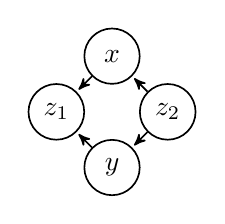
\begin{tikzpicture}[->,>=stealth',shorten >=1pt,auto,semithick]
  %\tikzstyle{every node}=[fill=none,draw=none]
 % https://tex.stackexchange.com/questions/445946/how-set-tikz-circle-radius-in-nodecircle
  \node[circle,draw, minimum size=20pt] (Z2) {$\adjustmentVar_1$};
  \node[circle,draw, minimum size=20pt] (X) [above right of=Z2] {$\decisionVar$};
  \node[circle,draw, minimum size=20pt] (Y) [below right of=Z2] {$\outcomeVar$};
  \node[circle,draw, minimum size=20pt] (Z1) [below right of=X] {$\adjustmentVar_2$};

  \path (Z1) edge  (X)
  (Z1) edge   (Y)
  (X) edge   (Z2)
  (Y) edge   (Z2);
\end{tikzpicture}

    }
    \innerblock{}{
        \centering
        \resizebox{22cm}{!}{
            \fontsize{10pt}{12pt}
            \pgfplotsset{every axis/.append style={xtick distance=.2, ytick distance=.2,width=7cm}}
            \begin{tikzpicture}[baseline]
    \pgfplotstableread[col sep=comma]{./data/4node_collider_summary.csv}{\datatable};
    \begin{semilogxaxis}[
        xlabel={No. of data points, $\nData$},
        ylabel={Parameter $\averageCausalEffect$},
        xmin=90,
        xmax=11000,
        legend style={
            font=\scriptsize, at={(0.5,1.10)},
            anchor=south,legend columns=-1},
    ]
        \addplot+ [ only marks, mark=*, mark size=1pt,
            error bars/.cd,
            y dir=both,
            y explicit] table [x=m_obs, y=ace_value, y error=q_ace_standard_error] {\datatable};
        \addplot+ [only marks, mark=*, mark size= 1 pt,
            error bars/.cd,
            y dir=both,
            y explicit] table [x=m_obs, y=ols_value, y error=q_ols_standard_error] {\datatable};
        \addplot [no markers] table [x=m_obs, y=ace_circ] {\datatable};
        \legend{{$\averageCausalEffectSet_{\confidenceLevel,\nData}$},{$\regCoefficientSet_{\confidenceLevel,\nData}$},{$\averageCausalEffectTarget$}}
    \end{semilogxaxis}
\end{tikzpicture}

        }
    }
}

\block[roundedcorners=0, linewidth=1mm, titleleft]{LiNGAM comparison}{
\innerblock{}{
    In one numerical experiment, we \textbf{compared our confidence intervals with DirectLiNGAM} from \emph{Shimizu et al. JMLR 12 (2011) 1225--1248} with boostrapping.
    Data was generated with \textbf{random true $\semCoeffMat$} different distributions for $\semNoise$, but with the same mean and covariance.
    }
\innerblock{}{
    Empirical coverage rate (CR) and the average Confidence Interval (CI) width for LiNGAM Bootstrap CI and $\blueGamma$ proposed in this article. The nominal CR was set to exceed $1-\alpha = 95\%$.
}
\innerblock{}{
    \centering
    \begin{tabular}{lllrr}
       \toprule
       Noise  & Method & CR    & Avg CI width & Avg $\averageCausalEffectEstN$ \\
       \midrule
       Normal & LiNGAM & 100\% & 2.01         & 0.64                           \\
              & our    & 99\%  & 0.15         & 1.79                           \\
       Exp    & LiNGAM & 92\%  & 0.08         & 1.77                           \\
              & our    & 100\% & 0.54         & 1.79                           \\
       Gumbel & LiNGAM & 85\%  & 0.07         & 1.77                           \\
              & our    & 100\% & 0.46         & 1.79                           \\
       \bottomrule
\end{tabular}

    }
}

\end{columns}
\end{document}